\chapter{Analyse dans le domaine temporel}
\label{chap:temporel}
	Jusque-là, nous avons principalement calculé la réponse de systèmes LTI en passant par le domaine fréquentiel, en utilisant les notions de fonctions de transfert, de transformée de Fourier et de Laplace. Cette approche permettait de calculer facilement cette réponse.
	Tous les calculs auraient pu être effectué en restant dans le domaine temporel à partir de la réponse impulsionnelle du système, que nous avions introduite au chapitre 2. Nous l'avions laissé de côté momentanément car son utilisation passait par un calcul relativement complexe, appelé produit de convolution. Nous allons le détailler dans ce chapitre.
	Nous pourrions croire que nous sommes en train de présenter un nouvel outil pour analyser l'effet d'un même système LTI. Nous allons voir au contraire que les concepts de fonction de transfert et de réponse impulsionnelle sont intimement liées.
	
	
	\section{Réponse impulsionnelle}
	
	\subsection{Définition}
	
	Comme nous l'avons vu dans le chapitre 2, il s'agit de la réponse d'un système LTI à une excitation impulsionnelle élémentaire, modélisée par une impulsion de Dirac. Sa connaissance permet de déterminer la réponse du système quelle que soit l'excitation appliquée à l'aide de la relation suivante, présentée au chapitre 2.
	\begin{equation}\label{Calcul_reponse_temporel_causal}
	y(t) = \int_{0}^{+ \infty} x(\tau) \cdot h(t-\tau)d\tau = x*h(t)
	\end{equation}
	\vspace{1\baselineskip}
	
	La réponse impulsionnelle et la fonction de transfert d'un système sont reliées par la transformée de Laplace. Plusieurs moyens permettent de le démontrer. Le plus simple consiste à exploiter le lien entre la multiplication et le produit de convolution : un produit de convolution dans le domaine temporel est équivalent à une multiplication dans le domaine fréquentiel.
	\begin{equation}\label{}
	y(t) =  h*x(t) ~\longleftrightarrow~Y(p)=H(p)\cdot X(p)
	\end{equation}
	
	Dans la prochaine partie, nous allons détailler les propriétés du produit de convolution et voir comment le mettre en œuvre pour résoudre l'équation \ref{Calcul_reponse_temporel_causal}.
	
	\subsection{Extraction de la réponse impulsionnelle}
	
	La réponse impulsionnelle d'un système peut s'obtenir de différentes manières. Expérimentalement, elle peut s'extraire en excitant le système par une impulsion élémentaire (tout du moins une forme s'en approchant). La réponse impulsionnelle sera directement la réponse du système. Une manière alternative est d'utiliser échelon unitaire a(t), parfois plus simple à générer qu'une impulsion. La réponse impulsionnelle est ensuite déduite en dérivant de la réponse indicielle.
	\begin{equation}\label{key}
	h(t)=\frac{da}{dt}
	\end{equation}
	
	La réponse impulsionnelle peut aussi être déterminée à partir de la fonction de transfert. Dans le domaine de Laplace, nous avons vu que la réponse impulsionnelle est égale à la transformée de Laplace inverse de la fonction de transfert. De même, dans l'espace des fréquences, la réponse impulsionnelle est la transformée de Fourier inverse de la fonction de transfert. Si l'expression de la fonction de transfert est disponible, on peut en déduire celle de la réponse impulsionnelle, à condition de savoir calculer sa transformée de Laplace ou Fourier inverse. Nous allons l'illustrer avec l'exemple suivant.
	
	
	
	\begin{minipage}[l]{0.6\linewidth}
		On reprend l'exemple du circuit RC (filtre passe-haut d'ordre 1) dans le chapitre 3, dont nous avions déterminé la fonction de transfert (H(p) et la réponse $u_{R}(t)$ à un échelon. On considère qu'initialement le condensateur C n'est pas chargé. Nous allons vérifier qu'on retombe sur la même réponse impulsionnelle à partir de ces deux informations. La fonction de transfert du circuit est donnée par :
	\end{minipage} \hfill
	\begin{minipage}[c]{0.50\linewidth}
		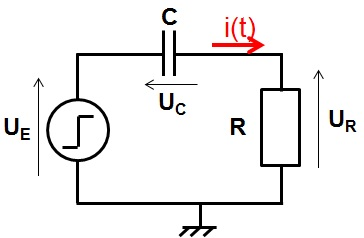
\includegraphics[scale=0.7]{images/circuit_RC_reponse_indicielle.jpg}	
	\end{minipage}

	\begin{equation*}
	H(p)=\frac{p}{p+\frac{1}{\tau}}~,~avec~\tau=RC
	\end{equation*}
	
	On obtient la réponse impulsionnelle h(t) du circuit à partir de la transformée de Laplace inverse de la fonction de transfert. On remarquera que le "p" au numérateur introduit un effet dérivateur. La transformée de Laplace de la dérivée d'une fonction nécessite de connaître la condition initiale. En $t=0^{+}$, comme le condensateur est initialement déchargé, la tension aux bornes de la résistance est égale à l'excitation : $u_{R}(0^{+})=\delta(t)$. 
	\begin{equation*}
	h(t)= \mathcal{L}^{-1}[p\frac{1}{p+\frac{1}{\tau}}]~\Longrightarrow~h(t)=u_{R}(0^{+})+\frac{d}{dt}(e^{-\frac{t}{\tau}})
	\end{equation*}
	\begin{equation*}
	h(t)=\delta(t)-\frac{1}{\tau}e^{-\frac{t}{\tau}}
	\end{equation*}
	
	
	A partir de la réponse à un échelon, en considérant un échelon unitaire qui démarre en t = 0, la réponse indicielle du circuit est donnée par : $a(t)=e^{-\frac{t}{\tau}} u(t)$. On en déduit la réponse impulsionnelle en dérivant la réponse indicielle. 
	\begin{equation*}
	h(t)=\frac{da(t)}{dt}=\frac{d}{dt}(e^{-\frac{t}{\tau}}\cdot u(t))
	\end{equation*}
	\begin{equation*}
	h(t)=e^{-\frac{t}{\tau}}\frac{du(t)}{dt}+\frac{d}{dt}(e^{-\frac{t}{\tau}})u(t)
	\end{equation*}
	\begin{equation*}
	h(t)=\delta(t)-\frac{1}{\tau}e^{-\frac{t}{\tau}}u(t)
	\end{equation*}
	
		
	
	Les deux approches nous donnent bien la même réponse.
	
	
	\section{Produit de convolution}
	\subsection{Définition}
	Soient deux fonctions x(t) et y(t) définis sur l'ensemble $L^{1}(\mathbb{R})$. Leur produit de convolution est donné par l'équation \ref{Convolution}.
	\begin{equation}\label{Convolution}
	x*y(t) = \int_{-\infty}^{+ \infty} x(\tau) \cdot y(t-\tau)d\tau 
	\end{equation}
	
	\subsection{Propriétés}
	Le tableau ci-dessous résume les principales propriétés du produit de convolution.
	
	\begin{table}[h!]
		\centering
		\caption{\label{Tab:Propriétés_convolution} Propriétés du produit de convolution}
		\begin{tabular}{|l|l|}
			\hline
			Commutativité & $x*y(t) = y*x(t) $ \\	
			\hline
			Distributivité & $z*(x+y)(t) = z*x(t)+z*y(t)$ \\	
			\hline
			Associativité & $z*(x*y)(t)=(z*x)*y(t)$ \\	
			\hline
			Retournement temporel & $z(t)=x*y(t)~\Rightarrow~z(-t)=x*y(-t)$ \\	
			\hline
			Point de départ & Si x(t)=0 pour $t<t_{x0}$ et y(t)=0 pour $t<t_{y0}$, alors $z(t)=x*y(t)=0$ \\ & pour $t<t_{x0}+t_{y0}$ \\
			\hline
			Point final & Si x(t)=0 pour $t>t_{x1}$ et y(t)=0 pour $t>t_{y1}$, alors $z(t)=x*y(t)=0$ \\ & pour $t>t_{x1}+t_{y1}$ \\
			\hline
			Durée & Soit x(t) et y(t) de durées finies $T_{x}$ et $T_{y}$. Si			 $z(t)=x*y(t)$,\\ &  la durée du signal z(t) est égale à $T_{z}=T_{x}+T_{y}$. \\
			\hline
		\end{tabular}	
	\end{table}
	
	Une propriété importante est l'équivalence entre le produit de convolution dans le domaine temporelle et la multiplication dans le domaine fréquentiel. Soient x(t) et y(t) deux signaux temporels, dont les transformées de Fourier sont X(f) et Y(f). La propriété précédente est donnée par (\ref{equiv_produit_conv_multiplication}). C'est cette propriété qui rend l'analyse fréquentielle intéressante dans l'étude des systèmes, puisque l'effet d'un système sur une excitation peut être déterminé par une simple multiplication, si les signaux sont exprimés dans le domaine fréquentiel. 
	\begin{equation}\label{equiv_produit_conv_multiplication}
	x*y(t)~\Longleftrightarrow~X(f)\cdot Y(f)
	\end{equation}
	
	La réciproque existe : la multiplication entre deux signaux dans le domaine temporel est équivalente à un produit de convolution dans le domaine fréquentiel (\ref{equiv_produit_conv_multiplication2}).
	\begin{equation}\label{equiv_produit_conv_multiplication2}
	x \cdot y(t)~\Longleftrightarrow~X*Y(f)
	\end{equation}

	Une dernière propriété importante est liée à l'impulsion de Dirac. Celle-ci correspond à l'élément neutre du produit de convolution (l'équivalent d'une multiplication par 1), comme le montre \ref{prod_convo_Dirac}. Cependant, si l'impulsion est décalée de $t_{0}$, alors le résultat du produit de convolution sera aussi décalée de $t_{0}$ (\ref{prod_convo_Dirac2}).
	\begin{equation}\label{prod_convo_Dirac}
	x(t)\cdot \delta(t)=x(t)
	\end{equation}
	\begin{equation}\label{prod_convo_Dirac2}
	x(t)\cdot \delta(t-t_{0})=x(t-t_{0})
	\end{equation}
	
	\textbf{\underline{Exemple :}}
	
	Soit un filtre caractérisé par une réponse impulsionnelle h(t). Il est excité en entrée par le signal $x(t) = 2\delta(t)+3\delta(t-1)-4\delta(t-2)$. Déterminez la réponse y(t) de ce filtre.\\
	
	En utilisant la propriété de distributivité du produit de convolution, on trouve facilement que la réponse du filtre est donnée par :
	\begin{equation*}
	y(t)=2h(t)+3h(t-1)-4h(t-2)
	\end{equation*}
	
	\vspace{1\baselineskip}
	
	
	
	\subsection{Mise en œuvre du produit de convolution}
	Dans cette partie, nous allons décrire une démarche permettant de calculer manuellement  le résultat d'un produit de convolution. Nous considérons un système causal dont on connait la réponse impulsionnelle h(t) ainsi que l'excitation x(t). On appelle y(t) le résultat du produit de convolution. L'opération considérée s'écrit donc :
	\begin{equation*}
	y(t)=h*x(t)=\int_{-\infty}^{+ \infty} h(\tau) \cdot x(t-\tau)d\tau 
	\end{equation*} 
	
	Pour déterminer chaque point en un temps $t_{0}$ donné de la fonction y(t), les différentes étapes à suivre sont les suivantes et sont illustrées à la figure \ref{Fig:Mise_oeuvre_prod_convo} :
	
	\begin{enumerate}
		\item Changement de variable : on remplace t par $\tau$.
		\item On trace $h(\tau)$.
		\item Pliage de la fonction $x(\tau)$ c'est-à-dire qu'on inverse l'axe temporel. On trace donc $x(-\tau)$.
		\item Décalage de la fonction pliée : on décale de $t_{0}$ la fonction $x(-\tau)$ pour tracer la fonction $x(t_{0}-\tau)$. Si $t_{0} > 0$, alors la fonction $x(t_{0}-\tau)$ est décalée vers la droite.
		\item Multiplication terme à terme de $h(\tau)$ et $x(t_{0}-\tau)$.
		\item Intégration du produit sur $\mathbb{R}$. L'aire sous la courbe donne $y(t_{0})$.
	\end{enumerate}

	Cette suite d'opérations est répétée pour obtenir les valeurs de tous les points de y(t).  
	
	\begin{figure}[h!]
		\centering
		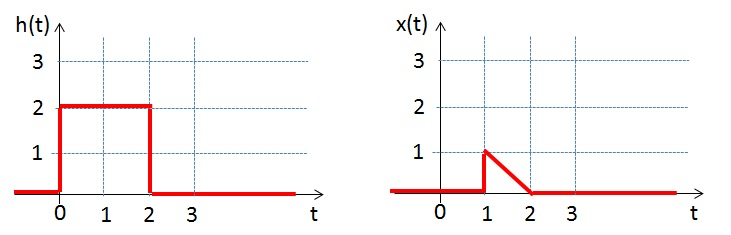
\includegraphics[scale=0.5]{images/Convolution_procedure_1}
	\end{figure}
	\begin{figure}[h!]
		\centering
		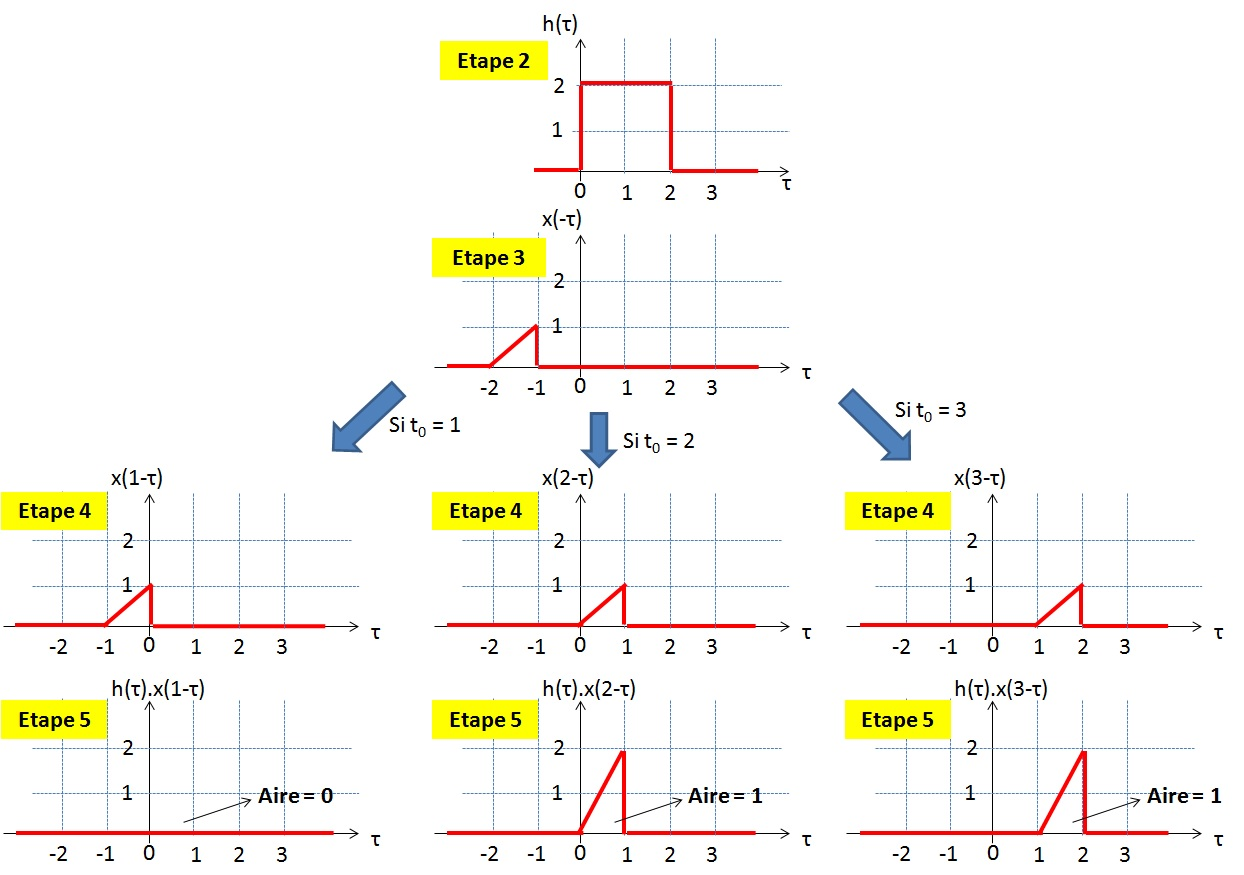
\includegraphics[scale=0.5]{images/Convolution_procedure_2}
	\end{figure}
	\begin{figure}[h!]
		\centering
		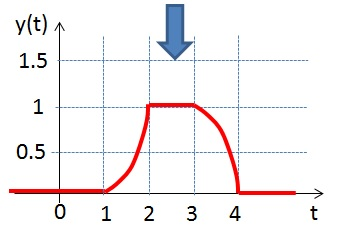
\includegraphics[scale=0.5]{images/Convolution_procedure_3.jpg}
		\caption{Illustration de la mise en oeuvre d'un produit de convolution}	
		\label{Fig:Mise_oeuvre_prod_convo} 
	\end{figure}
	
	
	\subsection{Durée du produit de convolution}
	
	Dans l'exemple graphique ci-dessous, les signaux h(t) et x(t) sont de durées finies, respectivement égales à 2 et 1. On remarque que celle du résultat du produit de convolution l'est aussi, et sa durée est égale à 3.
	Ce résultat se comprend à partir de la formule du produit de convolution, mais aussi par l'analyse graphique du calcul. De manière générale, si on réalise le produit de convolution de deux signaux x(t) et h(t) de durées $T_{x}$ et $T_{h}$, la durée $T_{y}$ du résultat y(t) du produit de convolution est donnée par \ref{Durée_prod_conv}. Si le signal x(t) démarre en $T_{x_{min}}$ et s'arrête en $T_{x_{max}}$ et si le signal h(t) démarre en $T_{h_{min}}$ et s'arrête en $T_{h_{max}}$, alors les bornes $T_{y_{min}}$ et  $T_{y_{max}}$ du signal y(t) sont données par \ref{Bornes_prod_conv}.  
	\begin{equation}\label{Durée_prod_conv}
	T_{y}=T_{h}+T_{x}
	\end{equation} 
	\begin{equation}\label{Bornes_prod_conv}
	T_{y_{min}}=T_{h_{min}}+T_{x_{min}}~~~~~~T_{y_{max}}=T_{h_{max}}+T_{x_{max}}
	\end{equation}
	
	\vspace{1\baselineskip}
	
	

	
	
	\section{Exemple : calcul de la réponse d'un filtre à partir de sa réponse impulsionnelle}
	
	On considère le filtre passe-bas ci-dessous (Fig. \ref{Fig:Circuit_passe_bas_convo}). La constante de temps RC du circuit est supposée être égale à 1, afin de simplifier les calculs. On suppose que le condensateur est initialement déchargé. On cherche la réponse temporelle y(t) du circuit lorsqu'il est excité par le signal x(t), présenté à la figure \ref{Fig:Excitation_passe_bas_convo}. Pour cela, nous allons mettre en œuvre le calcul du produit de convolution. Dans un premier temps, nous utiliserons la méthode graphique présentée ci-dessus. Dans un second temps, nous résoudrons directement l'intégrale \ref{Convolution}.
	
	\begin{figure}[h!]
		\centering
		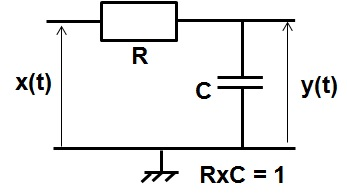
\includegraphics[scale=0.5]{images/Ex_passe_bas_convolution.jpg}
		\caption{Filtre passe-bas étudié}	
		\label{Fig:Circuit_passe_bas_convo} 
	\end{figure}

	\begin{figure}[h!]
		\centering
		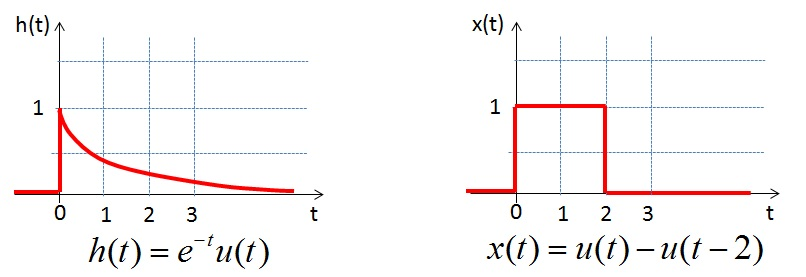
\includegraphics[scale=0.5]{images/Ex_excitation_passe_bas_convo.jpg}
		\caption{Réponse impulsionnelle du circuit (à gauche) et excitation (à droite)}	
		\label{Fig:Excitation_passe_bas_convo} 
	\end{figure}

	Il est d'abord nécessaire de calculer la réponse impulsionnelle h(t) du circuit. Elle peut facilement être déduite de sa fonction de transfert H(p).
	\begin{equation}\label{key}
	H(p)=\frac{1}{RC}\frac{1}{p+\frac{1}{RC}}~\Longrightarrow~h(t)=\mathcal{L}^{-1}[H(p)]=e^{-t}u(t)
	\end{equation}
	
	La réponse du filtre est obtenue en résolvant l'intégrale du produit de convolution ci-dessous. 
	\begin{equation}\label{convo_filtre_exemple}
	y(t)=h*x(t)=\int_{-\infty}^{+\infty}h(\tau)x(t-\tau)d\tau~~avec~t \in \mathbb{R}
	\end{equation}
	
	\vspace{1\baselineskip}
	\textbf{\underline{Méthode graphique :}}
	
	Commençons par utiliser la méthode graphique présentée dans la partie précédente pour déterminer l'allure et l'expression de la réponse du circuit. Sur la figure \ref{Fig:Ex_methode_graph_convo}, on a tracé la réponse impulsionnelle en fonction de $\tau$, ainsi qu'une version pliée et décalée de t de l'excitation ($x(t-\tau))$.  
	
	\begin{figure}[h!]
		\centering
		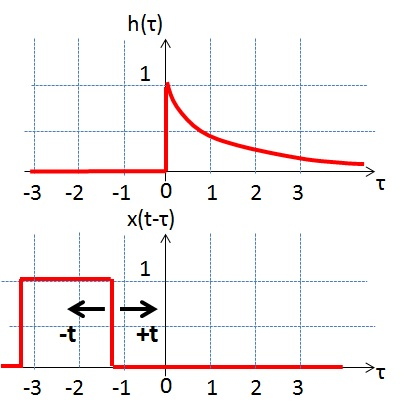
\includegraphics[scale=0.5]{images/Ex_methode_graph_prod_conv.jpg}
		\caption{Mise en œuvre graphique du produit de convolution pour le filtre passe-bas}	
		\label{Fig:Ex_methode_graph_convo} 
	\end{figure}
	
	Selon la valeur de t, l'intégrale du produit $h(\tau)x(t-\tau)$ prend des valeurs différentes. On distingue trois situations différentes :
	\begin{enumerate}
		\item si t < 0, alors $h(\tau)$ et $x(t-\tau)$ ne se recouvrent pas, donc $\int_{-\infty}^{+\infty}h(\tau)x(t-\tau)d\tau=0~~si~t<0$.
		\item si $0\leq t < 2$, seule une partie de $x(t-\tau)$ est recouvert par le début de $h(\tau)$. Le résultat du produit de convolution croit selon une exponentielle au fur et à mesure que t augmente. On a alors $\int_{-\infty}^{+\infty}h(\tau)x(t-\tau)d\tau=\int_{0}^{t}h(\tau)x(t-\tau)d\tau=1-e^{-t}$.
		\item si $t \geq 2$, alors $x(t-\tau)$ est complètement recouvert par $h(\tau)$. Le résultat du produit de convolution décroit exponentiellement quand t augmente. On a alors $\int_{-\infty}^{+\infty}h(\tau)x(t-\tau)d\tau=\int_{t-2}^{t}h(\tau)x(t-\tau)d\tau=e^{-(t-2)}-e^{-t}$.
	\end{enumerate}
	
	L'allure de la réponse du circuit est tracée sur la figure \ref{Fig:Ex_reponse_convo}. Puisque la réponse impulsionnelle est à durée infinie, c'est aussi le cas pour la réponse du filtre. Comme la réponse impulsionnelle et l'excitation démarre en t=0, c'est encore le cas pour la réponse y(t). Une expression peut aussi être déduite des résultats précédents :
	\begin{equation}\label{key}
	y(t)=(1-e^{-t})(u(t)-u(t-2))+(e^{-(t-2)}-e^{-t})u(t-2)=(1-e^{-t})u(t)-(1-e^{-(t-2)})u(t-2)
	\end{equation}
	
	\begin{figure}[h!]
		\centering
		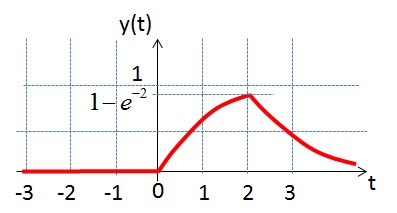
\includegraphics[scale=0.5]{images/Ex_reponse_prod_conv.jpg}
		\caption{Réponse du filtre passe-bas étudié}	
		\label{Fig:Ex_reponse_convo} 
	\end{figure}

	\vspace{1\baselineskip}
	\textbf{\underline{Calcul intégrale :}}
	
	Dans un second temps, nous essayons de résoudre directement l'intégrale \ref{convo_filtre_exemple}. En remplaçant $h(\tau)$ et $x(t-\tau)$ par leurs expressions respectives, on obtient :
	\begin{equation*}
	y(t)=\int_{-\infty}^{+\infty}e^{-\tau}u(\tau)\cdot(u(t-\tau)-u(t-(\tau-2)))d\tau~,~t\in \mathbb{R}
	\end{equation*}
	\begin{equation}\label{calcul_integrale_convo}
	y(t)=\int_{-\infty}^{+\infty}[e^{-\tau}u(\tau)u(t-\tau)-e^{-\tau}u(\tau)u(t-(\tau-2))]d\tau
	\end{equation}
	
	Dans l'intégrale \ref{calcul_integrale_convo}, on identifie deux termes. Calculons-les séparément.
	
	\begin{minipage}[l]{0.7\linewidth}
		Concernant le premier terme, on trouve :
		\begin{itemize}
			\item Si t < 0, alors $\int_{-\infty}^{+\infty}e^{-\tau}u(\tau)u(t-\tau)d\tau = 0$.
			\item Si $t \geq 0$, alors $\int_{-\infty}^{+\infty}e^{-\tau}u(\tau)u(t-\tau)d\tau = \int_{0}^{t}e^{-\tau}u(\tau)u(t-\tau)d\tau= 1-e^{-t}$.
		\end{itemize}
		On peut donc déduire l'expression suivante : $\int_{-\infty}^{+\infty}e^{-\tau}u(\tau)u(t-\tau)d\tau =(1-e^{-t})u(t)$
	\end{minipage} \hfill
	\begin{minipage}[c]{0.30\linewidth}
		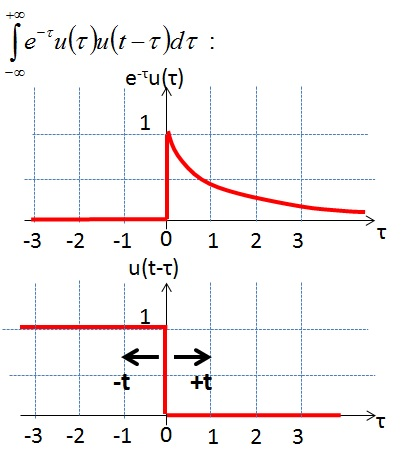
\includegraphics[scale=0.5]{images/Ex_integrale_prod_conv1.jpg}	
	\end{minipage}


	\begin{minipage}[l]{0.3\linewidth}
		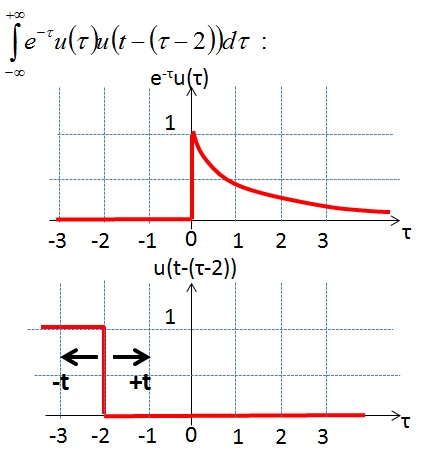
\includegraphics[scale=0.5]{images/Ex_integrale_prod_conv2.jpg}		
	\end{minipage} \hfill
	\begin{minipage}[c]{0.70\linewidth}
		Pour le second terme, on trouve :
		\begin{itemize}
			\item Si t < 2, alors $\int_{-\infty}^{+\infty}e^{-\tau}u(\tau)u(t-(\tau-2))d\tau = 0$.
			\item Si $t \geq 2$, alors $\int_{-\infty}^{+\infty}e^{-\tau}u(\tau)u(t-(\tau-2))d\tau = \int_{0}^{t-2}e^{-\tau}u(\tau)u(t-(\tau-2))d\tau= 1-e^{-(t-2)}$.
		\end{itemize}
		On peut donc déduire l'expression suivante : $\int_{-\infty}^{+\infty}e^{-\tau}u(\tau)u(t-(\tau-2))d\tau =(1-e^{-(t-2)})u(t-2)$
	\end{minipage}
	
	\vspace{1\baselineskip}
	
	En combinant les deux résultats, on en déduit l'expression de la réponse, qui correspond à celle déterminée avec la méthode graphique.
	\begin{equation}\label{key}
	y(t)=(1-e^{-t})(u(t)-u(t-2))+(e^{-(t-2)}-e^{-t})u(t-2)=(1-e^{-t})u(t)-(1-e^{-(t-2)})u(t-2)
	\end{equation}
	
	\vspace{1\baselineskip}
	
	On peut vérifier la validité de ce résultat en calculant la réponse à partir de la transformée de Laplace. On commence par calculer celles de la réponse impulsionnelle (càd la fonction de transfert) et de l'excitation.
	\begin{equation}\label{key}
	H(p)=\mathcal{L}[h(t)]=\frac{1}{p+1}
	\end{equation}
	\begin{equation}\label{key}
	X(p)=\mathcal{L}[x(t)]=\frac{1}{p}-\frac{e^{-2p}}{p}
	\end{equation}
	
	La réponse est ensuite obtenue en multipliant la fonction de transfert et l'excitation dans le domaine des fréquences complexes.
	\begin{equation*}
	Y(p)=H(p)\cdot X(p)=\frac{1}{p(p+1)}-\frac{e^{-2p}}{p(p+1)}=(\frac{1}{p}-\frac{1}{p+1})(1-e^{2p})
	\end{equation*}
	\begin{equation*}
	y(t)=\mathcal{L}^{-1}[Y(p)]=(1-e^{-t})u(t)-(1-e^{-(t-2)})u(t-2)
	\end{equation*}
	
	\vspace{1\baselineskip}
	
	
	
	\section{Exercices}
	
	\subsubsection{Exercice 1}
	
	Déduire les réponses impulsionnelles des systèmes décrits par les fonctions ci-dessous :\\
	a. $G(p)=\frac{1}{p(p+2)}+\frac{1}{2}(\frac{e^{4}}{p+2}-\frac{1}{p})e^{-2p}$ \\
	b. $H(j\omega)=\frac{2j\omega}{2+j\omega}$\\
	c. $a(t)=t^{2}u(t)$ où a(t) est la réponse indicielle \\
	d. $a(t)=u(t)(2-e^{-t})$ où a(t) est la réponse indicielle\\
	
	\subsubsection{Exercice 2}
	
	Calculez les produits de convolution suivants : \\
	a. $e(t)=u*u(t)$ avec $t \in \mathbb{R}$\\
	b. $f(t)=sin(t)*\Pi_{2a}(t)$ avec $t \in \mathbb{R}$\\
	c. $g(t)=cos(t)*\Pi_{2a}(t)$ avec $t \in \mathbb{R}$\\
	d. $h(t)=\Pi_{2a}(t)*e^{-bt}$ avec $t \in \mathbb{R}$\\
	e. $m(t)=(\delta(t-1)-\delta(t-2))*(u(t+1)-u(t-1))$ avec $t \in \mathbb{R}$\\
	
	\subsubsection{Exercice 3}
	
	On considère les fonctions h(t) et x(t) dont le profil est représenté ci-dessous.\\
	\begin{figure}[h!]
		\centering
		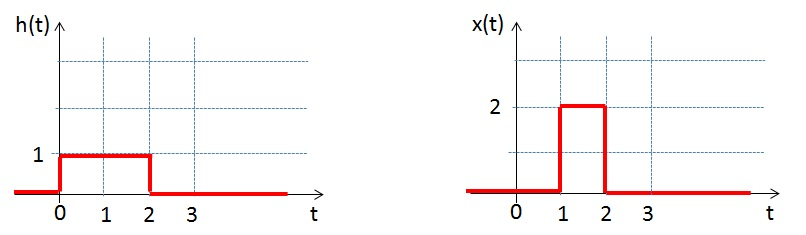
\includegraphics[scale=0.5]{images/Courbes_TD_Convolution_2.jpg} 
	\end{figure}
	
	1. Proposez une expression mathématique pour ces deux fonctions.\\
	
	2. On note y(t) le résultat du produit de convolution de x(t) et h(t). Déterminez l'expression de y(t) en calculant directement le produit de convolution. Tracez l'allure de cette fonction.\\
	
	3. En utilisant la transformée de Laplace, vérifiez la validité du résultat précédent.\\
	
	4. Même chose en utilisant la transformée de Fourier.\\
	
	\subsubsection{Exercice 4}
	On considère un filtre linéaire à temps invariant dont la fonction de transfert est donnée par $H(\omega)=\frac{j\omega}{1+j\omega}$. \\
	
	1. On l'excite à l'aide d'un signal échelon. Calculez la réponse du filtre en utilisant sa réponse impulsionnelle. Esquissez sa forme temporelle.\\
	
	2. Même question si on excite le filtre à partir du signal $e(t)=u(t)-u(t-2)$.\\


	
	\subsubsection{Exercice 5 - Convolution de spectre}
	
	On considère deux signaux, définis par les fonctions $f_{1}(t) = cos(\omega_{1}t) et f_{2} = cos(\omega_{2}t)$. \\
	
	1. Déterminez l'expression du spectre du signal $f(t)=f_{1}(t)\cdot f_{2}(t)$ (on prendra $\omega_{1} > \omega_{2}$). Représentez-le graphiquement.\\
	
	2. Même chose avec $f_{2}(t) = sin(\omega_{2}t)$.\\
	
	3. Même chose avec $f_{2}(t) = sinc(t)$.\\
	
	4. Conclure sur l'effet de la multiplication par un signal sinusoïdal.\\

	
	
	\subsubsection{Exercice 6}
	
	On considère la fonction porte $\pi_{[-a;a]}(t)=\pi(t)$ avec $a \in \mathbb{R^{*}}$.\\
	
	1. Calculez le produit de convolution $s(t)=\pi(t)*\pi(t)$.\\
	
	2. Calculez la transformée de Fourier $\Pi(f)$ de la fonction $\pi(t)$. En déduire l'expression de la transformée de Fourier S(f) de la fonction s(t).\\
	
	3. Soit le signal $l(t)=\pi(t) \cdot \pi(t)$. Calculez la transformée de Fourier L(f) de la fonction l(t).\\
	
	On pose a = 0.5. On considère $t \in \mathbb(R)$.
	
	4. Calculez le produit de convolution $p(t)=\pi(t)*\pi(\frac{t}{2})$.\\
	
	5. On considère les fonctions définies par $s_{1}(t)=\pi(\frac{t-1}{2})$ et $s_{2}(t)=s_{1}(t)-s_{1}(t-2)$. Tracez $s_{1}(t)$ et $s_{2}(t)$. Calculez le produit de convolution entre $s_{1}$ et $s_{2}$.
	
	\vspace{1\baselineskip}
	
	\subsubsection{Exercice 7 - Échantillonnage}
	
		On considère le circuit de principe ci-dessous, formé d'un interrupteur idéal et appelé échantillonneur. x(t) est le signal d'entrée, h(t) le signal de commande d'ouverture/fermeture de l'interrupteur, et y(t) le signal de sortie. L'interrupteur est ouvert lorsque la commande est nulle. Il se ferme lorsque la commande h(t) = 1.
	Dans cet exercice, on considère que la commande est formée par un peigne de Dirac de période T. Dans un premier temps, le signal d'entrée est une fonction sinus cardinal, tel que $x(t)=A\cdot \frac{sin(\pi \frac{t}{\tau})}{\pi \frac{t}{\tau}}$.
	
	\begin{figure}[h!]
		\centering
		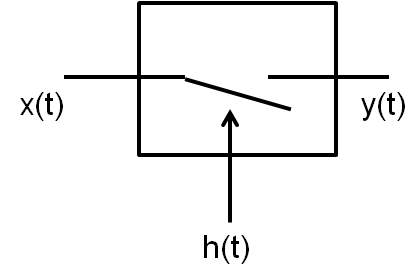
\includegraphics[scale=0.6]{images/Echantillonneur.png} 
	\end{figure}
	
	
	1. Donnez la relation entre les signaux de sortie, d'entrée et de commande.\\
	
	2. Tracez l'allure du signal de sortie. Le nom d'échantillonneur donné au circuit est-il justifié ? Sa présence est-il nécessaire dans un circuit de traitement du signal ?\\
	
	3. Donnez les transformées de Fourier des signaux x(t) et h(t) ? Esquissez leur spectre (en amplitude).\\
	
	4. Déterminez la transformée de Fourier du signal y(t). Esquissez son spectre dans le cas où T << $\tau$, puis dans le cas où T > $\tau$.\\
	
	5. Est-il possible de retrouver le signal x(t) à partir de l'acquisition du signal y(t). Comment et sous quelles conditions ?\\
	
	6. Pourquoi est-il nécessaire de limiter la bande passante des signaux à échantillonner ?
	